\section{Analisi del Prodotto}
\subsection{Scopo del prodotto}
Lo scopo del prodotto che si andrà a realizzare nel corso di questo progetto è quello di costruire un prototipo di
template di e-commerce basato su tecnologie serverless, utilizzando principalmente tecnologie cloud \textit{AWS}.
Una volta sviluppato, sarà necessario istanziare il prodotto inserendo prodotti e categorie come se fosse in uso
da un venditore, per eseguire la validazione finale.

\subsection{Analisi della struttura}
Il progetto \textit{\glock{EmporioLambda}} è strutturato in:
\begin{itemize}
    \item \textbf{\glock{EML-FE}}: è il componente per il front-end del sito: deve occuparsi di servire la pagina web richiesta dall'utente. Il suo compito è di effettuare il pre-rendering della pagina lato server ad ogni richiesta;
	\item \textbf{\glock{EML-BE}}: è il componente per la parte di back-end della piattaforma. Si occupa di:
	\begin{itemize}
        \item implementare la \textit{\glock{business logic}} dell'applicazione;
        \item gestire i dati dell'applicazione (e.g. ordini, informazioni sui prodotti e sui clienti);
        \item gestire lo stato del carrello;
        \item integrare i servizi di terze parti.
    \end{itemize}
	\item \textbf{\glock{EML-I}}: è il modulo per l'integrazione dei servizi di terze parti, utili ad esempio per le operazioni di pagamento e per l'autenticazione degli utenti;
	\item \textbf{\glock{EML-MON}}: la sua funzione è fornire il set di strumenti necessari per il monitoraggio del sistema da parte dell'amministratore.
\end{itemize}

\subsection{Attori}
Gli attori che il gruppo ha individuato sono i seguenti:
\begin{figure}[H]
    \centering
    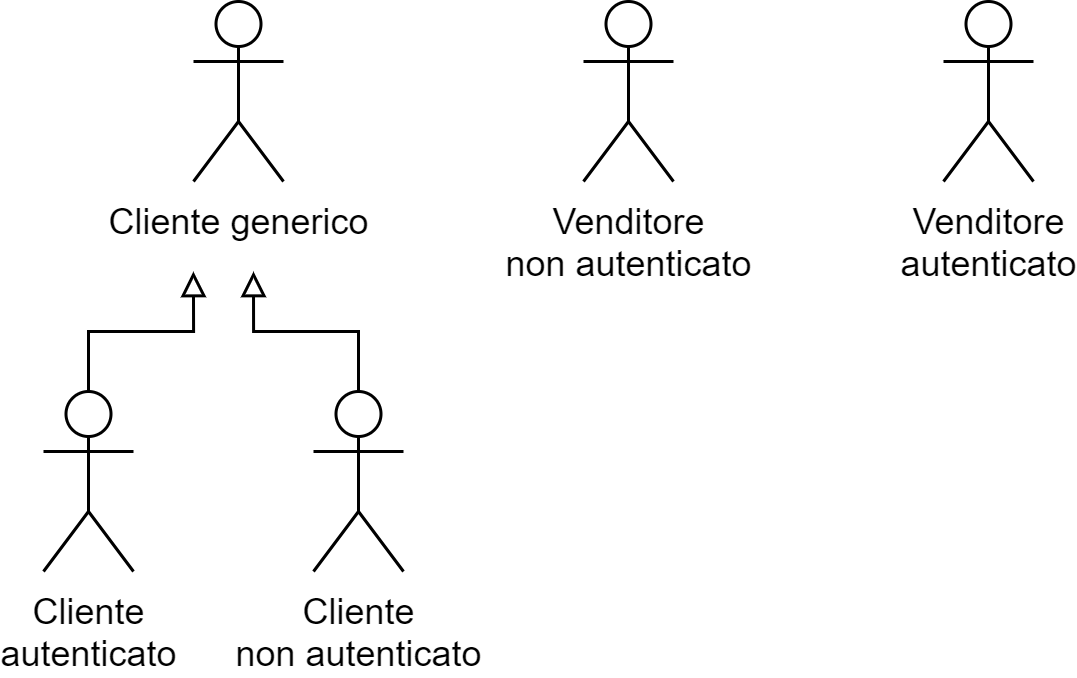
\includegraphics[width=32em]{res/images/UC/attori.png}
    \caption{Diagramma attori} 
\end{figure}
\subsubsection{Attori Principali}
\begin{itemize}
    \item \textbf{Cliente generico:} cliente che naviga la piattaforma e può usarne la maggior parte delle funzionalità come navigazione, ricerca, aggiunta al carrello del prodotto, acquisto. Si differenzia in: 
    \begin{itemize}
        \item \textbf{cliente autenticato:} cliente che ha superato la fase di login e può accedere alle funzionalità riservate ai clienti autenticati;
        \item \textbf{cliente non autenticato:} cliente che non ha ancora eseguito il login oppure non è ancora registrato alla piattaforma. 
    \end{itemize}
    \item \textbf{Venditore non autenticato:} venditore che non ha ancora effettuato il login.
    \item \textbf{Venditore autenticato:} venditore che ha effettuato il login con successo. Può accedere a tutta la sezione riservata della piattaforma dove può amministrare tutte le funzionalità (amministrazione prodotti, amministrazione categorie, amministrazione piattaforma).
\end{itemize}
